\section{Introduction}
This paper is about an academic project born to be an efficient solution for the CINI\footnote{Consorzio Interuniversitario Nazionale per l'Informatica} 2017 Challenge on smart cities illumination systems. In particular, the goal was to prototype and test a solution which was capable of (near) real-time data stream processing for monitoring records from street lamps, lumen sensors co-located with the street lamp itself and from traffic data produced by third-party APIs. We will explore this solution for the following use case: in a smart city context it is necessary to guarantee the maximum efficiency from lamps consumption while providing an optimal illumination within safety limits for pedestrians and drivers and according to local traffic intensity. To achieve that, it is necessary to project a grid of smart lamps capable of tuning their light level according to the right amount of energy necessary to provide city aware, safe and green consumption levels. This grid must be powered and managed via a reliable, highly available, processing-capable control system. Introducing Project Ember.


\section{Frameworks and Tools}
We structured our environment using at first a publish/subscribe architecture with street lamps, lumen and traffic sensors as publishers and the stream processing framework as subscriber. 

\subsection{Data stream processing}
The Apache Software Foundation makes available different alternatives, each one a refined version of the previous: Apache Storm is one of the most used data stream processing framework on the market and one of the most supported as well; Apache Spark is a refined version of Storm even though it is limited to fewer programming languages (Java, Scala and Python); Apache Flink\footnote{Apache Flink official page: https://flink.apache.org/} is the most recent project among the three and the most advanced. Flink gives the programmer the possibility to define just the topology of the operators, how they are linked, or how to set the windows timing (based upon the event time or upon the processing time spent inside the system). Flink handles the under-the-hood engine: multithreading, synchronization, parallelism, availability, cluster management. We chose the latest stable release of Apache Flink, 1.2.0, which comes with a well written documentation as well as multiple connectors for the most popular MOM\footnote{Messages Oriented Middleware} and storages. Flink calls a Source the very component that produces data and Sink the one that takes the processed data in order to store or to route them to another entity.

\subsection{Connectors}
To achieve scalability we had to analyze several options to let connect our Flink topology to messages routers and to the persistence level. The MOM chosen was Apache Kafka\footnote{Apache Kafka documentation: https://kafka.apache.org/documentation} works seamlessly with Flink thanks to the included connector plugins giving the possibility to simply personalize the connection according to our preferences: in particular in this solution Kafka is our preferred Source to handle data from the sensors. Talking about the Sinks, Flink supports many platforms and Kafka can be one of them (for example for the control output), but in order to persist and manage our data we wanted to use also a modern platform capable of organizing data for (near) real-time purposes.

\subsection{Persistence level}
A NoSQL approach was mandatory to us, to collect dynamic unstructured data typical of a sensor network, so we analyzed different products: in particular Elasticsearch\footnote{Elasticsearch official page: https://www.elastic.co/products/elasticsearch} and Apache Cassandra. We chose Elasticsearch, as it is fully supported (not its last version indeed) by Flink 1.2.0 and it is a flexible, easy-to-deploy database with RESTful APIs. It leverages the ability to perform complex queries, even geographical and lexical ones, with good performances and scalability options. Elasticsearch is part of the Elastic Stack built by Elastic.co which makes available another useful tool for visualizing data stored in Elasticsearch, Kibana\footnote{Kibana official page: https://www.elastic.co/products/kibana}.

\subsection{Extras}
To develp a local control unit to manage the city grid we used Flask and Redis. Flask\footnote{Flask official page: http://flask.pocoo.org/} is a micro-framework for Web Server built in Python and Redis\footnote{Redis official page: https://redis.io/} instead is simple and efficienty key-valye data store and works as a database, cache and message broker. Redis serves us as a cache, allowing us to interact with control unit history with it with very simple APIs via the endpoints exposed by Flask.

\subsection{Programming languages}
Java is the programming language that links all these components together being used by Flink as well as Scala, such as Elasticsearch APIs. We also used Python for the control unit development as well as to realize the simulated data source for testing.


\section{Architecture overview}
In this section we will cover how the system communicates between each of its components and modules and the assumptions we made to prototype and test the architecture. In \hyperref[fig:ember_architecture]{figure 1} a high-level architecture overview is provided. Before proceeding, we want to focus on the output from the real-time\footnote{We will define the system as "real-time" in this paper even if is not validated for such a control system, but it is capable of near real-time data streams processing} control system: it is produced into the MOM and consumed by control units (how will be discussed later), closing a feedback loop. This behavior and the capabilities to maintain high-availability across the clusters make the system itself near to the features of an autonomic system.
\begin{figure}[!b]
\begin{center}
	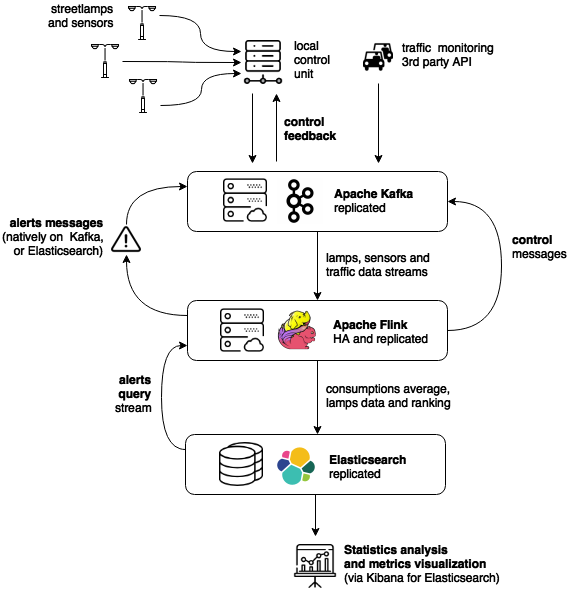
\includegraphics[scale=0.35]{img/ember_architecture}
	\caption{Project Ember architecture overview}
	\label{fig:ember_architecture}
\end{center}
\end{figure}

\subsection{Sensors network}
First of all let us consider how the sensors network sends its data to the control system. According to project specifications the street lamps sends to the system a JSON formatted string containing all the information their microcontrollers collect as a tuple\footnote{in particular a unique integer id, address and model, consumption, intensity level, power on status and last replacement (as a timestamp in seconds) plus the timestamps in seconds of the instant the tuple was sent}. Those data are sent every 10 seconds. A lumen sensor is placed on the lamp and it sent data with same rate as well giving us information about the daylight luminosity level and the id of the lamps it is placed upon.

\subsection{Control unit}
The control unit gives us the possibility to create a new indirection level that is placed among the lamps and Flink. The lamps talk, using the city intranet, to the local control unit which maintains a mapping between the lamps ids and their IP addresses inside the local city network. The control unit manage the correct routing of the messages from the lamps to the stream processing operator via Kafka, as well as the control feedback received via the same MOM: to made it available we added to the JSON representing the lamp a control unit identifier as an alphanumeric string. This solution was introduced both for the indirection it introduces and the plug-and-play registration of each new lamp via RESTful APIs, as well as the capability to store the sensible data at the edge of the network to decrease latency, giving us some features of the fog computing paradigm.

\subsection{Apache Kafka cluster}
To handle the thousands of data necessary to manage the infrastructure, we thought to use a cluster of replicated nodes running the same Apache Kafka instance, using Apache Zookeeper\footnote{Apache Zookeeper official page: https://zookeper.apache.org} to maintain the cluster available via redirection from a public IP. As we will see later, the MOM allows us to register topics for lamps, sensors and traffic monitoring data to retrieve them as a stream in Flink, and to create automatically topics for each control unit in order to retrieve the control feedback for each sector of the city grid. In addiction we included the possibility to route via Kafka alerts messages (to be consumed later by a custom operator).

\subsection{Apache Flink cluster}
This is the core of the architecture. The Apache Flink framework was used to create a data stream (near) real-time processing system to handle the thousands of tuples per seconds from the city grid and to produce for each of them a control output, as well as aggregations by streets or identifiers to produce statistics, ranks (by last replacement) and to store them for further analysis. Flink is also used to continuously monitor data from Elasticsearch and to produce alerts for any kind of failures that is collectable from each lamp history. To provide the necessary resilience and to let the processing system to scale, it is intended to be deployed as an highly-available cluster, composed of a \texttt{JobManager} (replicated and managed via Apache Zookeeper), acting as a master, and some \texttt{TaskManagers}, acting as slaves, into which is replicated every stream according their computational power (one core is one execution slot), producing several degrees of parallelism proportional to the cluster size. Moreover, any transition of a set of parallelized streams is handled via the \texttt{JobManager} node into a single time window to perform any bath-like computation (as for example average computation).

\subsection{Elasticsearch and Analytics}
The ranks, the consumption mean by id and by address, have to be visualized and showed in real-time, so Elasticsearch comes in help. Flink offers an interface for Elasticsearch, that, simply providing the cluster configuration, connects to it and allows to send data in byte encoded json format strings. Elasticsearch organizes data by so called Indexes and Types. The Index is the equivalent of Database in a NoSQL approach and the Types the equivalent of Tables. Elasticsearch keeps tracks of data assigning them a mapping table so it can be capable of understand primitives or complex data types. Kibana comes in our help for representing them. By a simple file of configuration you can use Kibana to create your own dashboard by defining all the data to be analyzed specifying the Type it has to use, how rearrange the attributes, how to order and in which style visualize them. Elasticsearch and Kibana has been designed to easily interact each other, keeping synchronized the dashboard across Kibana clients, and be simply deployed as well. Elasticsearch can be extended without any amount of effort, simply defining new nodes for the cluster and joining the master node. Elasticsearch serves also a particular role: being designed as a RESTful engine as well, it allows to specify complex query and resolves them efficiently, using at its core Apache Lucene, an open source machine learning library.


\section{DATA STREAM PROCESSING}
In this section we will introduce and cover the data stream processing system. As we introduced before, it is based upon Apache Flink 1.2.0 (latest stable release). Before exploring the topology we used, we must introduce some basic concepts.

\begin{figure}
\begin{center}
	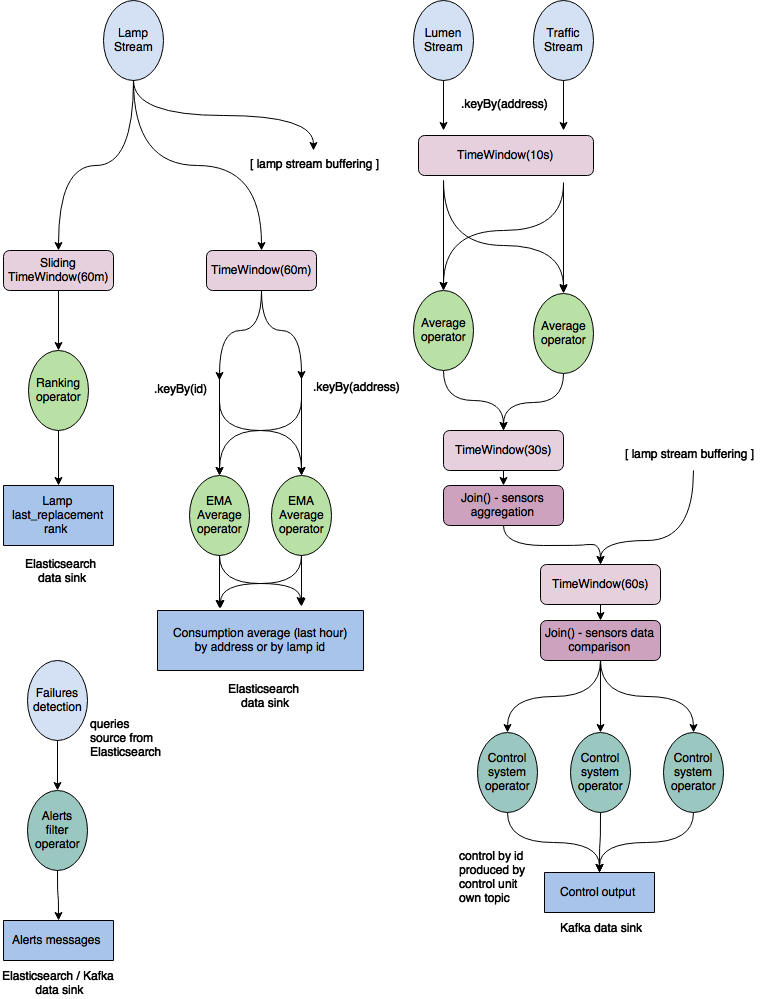
\includegraphics[scale=0.3]{img/ember_topology}
	\caption{Project Ember topology}
	\label{fig:ember_topology}
\end{center}
\end{figure}

\subsection{Basic concepts}
Apache Flink is based on the concept of \texttt{DataStream} (it also supports datasets but they are not used in this project), which is an immutable collection of data where the number of elements is unbounded. 
DataStreams are produced by the \texttt{ExecutionEnvironment}, which is automatically created by the framework locally or distributed according to the cluster size defined in Flink configuration parameters. To create a data stream and to store it, the environment is bounded to a set of data \texttt{Sources} and \texttt{Sinks}, whose implementation we will discuss later.

In this project we needed to performa a real-time computation on several kinds of data sources, so we used the \texttt{DataStream API} made available by Apache Flink framework. This decision allowed us to create streams grouped by some specific attribute of the elements (as a \texttt{Key}), to aggregate them into \texttt{TimeWindows} and to perform later a \texttt{Join} operation to compute results on specific time intervals. 

Apache Flink is built to introduce very low latency for an high throughput and to allow the developers to create a natural flow control decoupling the logic behind the stream processing from the deployment itself. In other words, it is built to be efficient and to let developers concentrate their efforts in building the topology of the system regardless the machines the system will run upon.

\subsection{Topology}
As we said, Apache Flink supports parallelism of the streams processing according to task slots available per-machine of its cluster. Describing the topology we will assume a certain degree of parallelism which is not necessary to run the system locally (accurate performances analysis will be discussed in another section).

In \hyperref[fig:ember_topology]{figure 2} is represented the high level schema for our topology (exception made for the data sink which update lamp status in Elasticsearch). We can note that the streams produced are four, three coming from sensor sources attached to the execution environment (via Apache Kafka custom connectors), while the last one is a custom source that generates anomalies arouse from the queries to the Elasticsearch lamps index and then perform a failure check, producing in output alerts messages.
It is interesting to note the replication of the more CPU-consuming tasks, as well as the group of streams tuples by a specific key to perform transformations and specific forwarding to dedicated operators.

As it is clear from the topology schema, we made use of time windows to buffer, to aggregate and to analyze specific time intervals of the streams. This introduced overhead increasing the time spent by one record into the system, but it allowed us to reduce the jitter on output messages and stabilize the entire control system: using windows we can easily compare datasets of the same dimensions and properties decoupling the arrival from the service process of our operators network.

\subsection{Sources and Sinks}
Sources are where the topology takes its inputs. A custom source can be attached to the topology via the execution environment calling \texttt{StreamExecutionEnvironment.addSource(sourceFunction)}. In particular a source function generated a datastream that will be transformed and forwarded to the correct operators in the topology. We used sources from the Kafka connectors made available by Apache Flink to continuously consume from the topics \texttt{lamp, lumen, traffic} to read data from the sensors, and a custom source function iterating over queries made to Elasticsearch in order to recover anomalies found in lamps history. Respectively we used the \texttt{FlinkKafkaConsumer101} to receive messages routed via the Kafka cluster, and the customized \texttt{EmberElasticsearchAlertSource} which is powered by the tuple collector made available by the execution environment.

Sinks are, on the other hand, the way Apache Flink consumes the data streams and forward them to external systems or print them out in a file. In this implementation we used two custom sinks, extending the built-in connectors: one is the \texttt{EmberKafkaProducer} and one is the \texttt{EmberElasticsearchSinkFunction}. In particular the latter is extended for each use case, from the simple lamp history update operations to the update of the ranks of the life-expiring lamps. The first producer, instead, is a \texttt{SinkFunction} which is extended in the \texttt{EmberKafkaControlSink}: in this case we used the feature of the Java Kafka API to select and create a topic into the MOM, that was particularly useful to route for each lamp its control output labelling each feedback with the lamp's own control unit identifier.
\begin{figure}
\begin{center}
	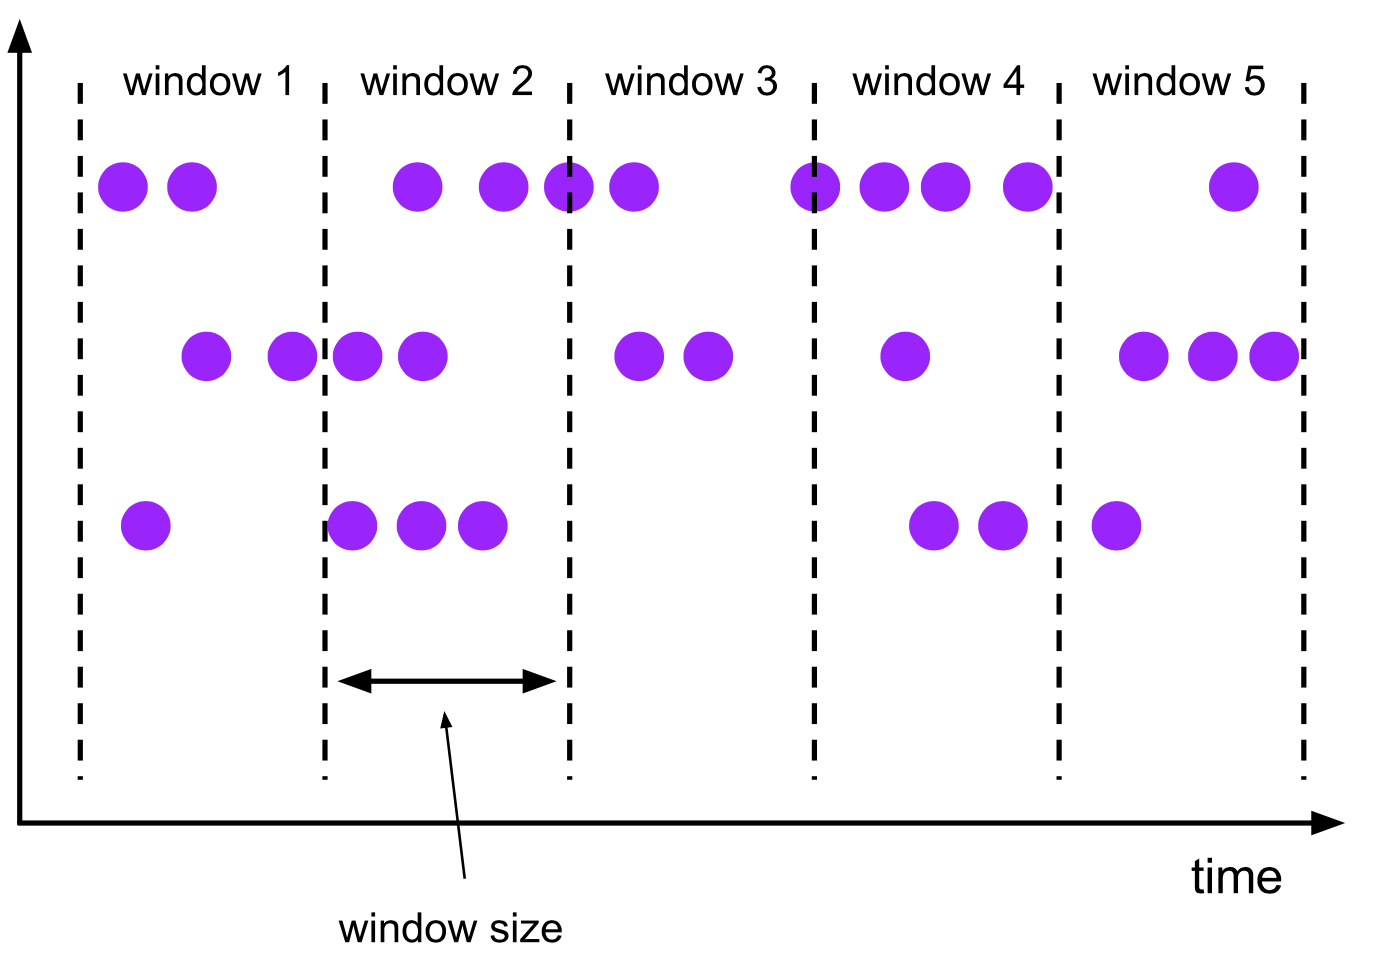
\includegraphics[scale=0.25]{img/flink_windows}
	\caption{Apache Flink tumbling windows}
	\label{fig:flink_windows}
\end{center}
\end{figure}

\begin{figure}[!b]
\begin{center}
	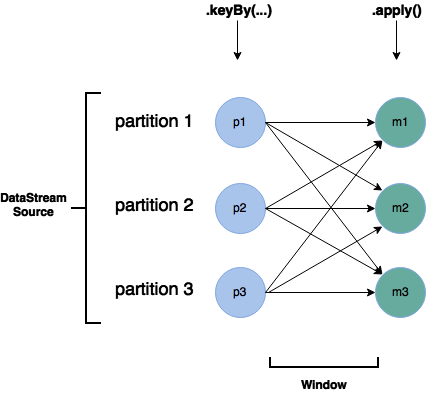
\includegraphics[scale=0.40]{img/ember_keyedstream}
	\caption{An example of Project Ember operator}
	\label{fig:ember_operator}
\end{center}
\end{figure}

\subsection{Data aggregation}
The large part of our stream processing system is based upon the class of \texttt{TumblingWindow} and \texttt{KeyedStream}\footnote{Windows on keyed streams: https://ci.apache.org/projects/flink/flink-docs-release-1.2/dev/windows.html}. In fact, as we can see from our topology, the great part of the operators is composed of a keyed streams (grouped by an attribute of the records they collect) being windowed for an amount of time to compute over them a custom \texttt{JoinFunction}. There are exceptions, as the ranking, that we will cover later, and the alerting system and history-update by Elasticsearch sink whose don't require such a complexity and are simply buffered and iterated upon in order to collect new data streams. 

Before going deeper with our system, let we analyze the sample Java code used:
\begin{lstlisting}[language=Java,basicstyle=\small]
stream
    .keyBy(...)      <-  required: "selector"
    .window(...)     <-  required: "assigner"
    .apply(...)      <-  required: "function"

stream
    .join(...)       <-  required: "datastream"
    .where(...)      <-  required: "selector"
    .equalTo(...)    <-  required: "selector"
    .window(...)
    .apply(...)
\end{lstlisting}
As we seen in the topology, we used a specific selector to partition the streams by id, or address (\hyperref[fig:ember_operator]{figure 4}).  Then we will buffer the streams and their partitions according to a \texttt{Watermark} assigned by the source, typically the timestamp associated with the event generation, into windows which size is configurable (\hyperref[fig:flink_windows]{figure 3}). It is important to note here that the developer must pay attention to specify a \texttt{EventTimeTumblingWindow} for events generated from the source and not already processed by the system, and \texttt{ProcessingTimeTumblingWindow} for the latter ones. In particular, for a window following a previous aggregation (as it is for the control operator) we will use the \texttt{ProcessingTime} to maintain the system coherent with its internal clock and preserving the original event generation time assigned by watermarks definition.

Finally we can choose which operation perform calling the \texttt{apply()} function, for example a moving average computation by lamp identifier or lamp address. We can also perform a \texttt{join()} over a new stream using a particular window in order to aggregate different data records in a single tuple and made them available for further operations, as it is performed twice in the control system flow.

\subsection{Control system}
The core of the control system is the flow which takes the sensors data streams, buffers and aggregates them twice (by their common selector and with data from lamps) and produces a control output which is sent to Kafka cluster to be consumed by control units.

In particular, the light sensors and traffic records are partitioned via their address and then buffered into a 10 seconds (event time) window. This is made to let the system behave according a unique step, the ten-seconds-interval assumed in the project specifications. Then a simple arithmetic average is performed on the records received, before aggregating the two streams by the address attribute. Then a new 30 seconds (processing time) window is used to aggregate those new tuples with the raw data from the lamps and compare them. Every minute the control system produces and filter by lamp single identifier an optimal control value using the formula:
	$$I = \frac{L_l*C_u}{A_l}$$
where the optimal intensity level, according the lumen level per square area, is proportional to an attenuation factor assumed unitary in this implementation and inverse to the diffusion area.

The optimal intensity level is calculated via the previous formula, which takes as arguments the level measured from the lamp and lumen sensors, and it is normalized using the percentage of traffic and safety limits. The concept idea is to define an optimal value that allows the city grid to avoid excesses between lamp consumptions, but guaranteeing an optimal level in case of intense vehicles traffic and a safety level for low traffic zones to secure pedestrian traffic. In addiction, working on lumen sensors, we can achieve the goal to find an optimal value even in scarce weather conditions, according the light sensors readings (for example in a cloudy or rainy day).

Finally the output produced is a \texttt{DataStream<StreetLamp>} which is produced into a topic equal, for each lamp, to its control unit alphanumeric identifier.

\subsection{Statistics}
An important aspect of this project was to compute on the fly useful statistics on the smart city grid. We provided three different approaches for three different use cases.
\subsection*{Expiration ranking}
To produce an always updated rank of the ten lamps most in danger for end-of-life expiration, we used an \texttt{EventTimeSlidingWindow} which takes care to perform a per-hour rank upon the last replacement (as a timestamp) attribute from the lamps records.
\subsection*{Last hour consumption}
The system is also capable to track on basis of a one-hour-step the consumption average, which is then stored into Elasticsearch for security reasons (if the system is terminated or must be restarted the persistence level will take trace of the history, losing just the last hour measurements). To perform a computation which is focused to give the most reasonable result, we used an exponential moving average:
$$S_t = \alpha*Y_t + (1 - \alpha)*S_{t-1}$$
$$\alpha = 0.8$$
giving preference to the last results from the hour-long buffer. The average is computed by address and by id for further analysis.
\subsection*{Data history}
An important aspect of a project like Project Ember is to visualize data. Even if we covered a lot how Elasticsearch works and how Kibana is integrated, a continuously updated history for the lamps values, as well as last hour consumptions, let us build useful dashboards to monitor in (near) real-time the system overall status.

\subsection{Alerts}
A useful feature of Project Ember is to provide a customizable preferential access for operators to the anomalies detection system. Once a configurable time, a query is performed to Elasticsearch cluster using its Apache Lucene based core to check on the entire lamps index for anomalies, such as out of range luminosity levels, electrical failures (lamps not reachable) of the control unit or the lamp, or lamp life expiration overflowed limits: no effort for the stream processing system. It must only handles those results and produce them via a custom sink on Elasticsearch or Kafka clusters, according the final user configuration: dashboard-based approach or not.

\subsection{Configuration}
Most of the parameters we quoted describing the stream processing and control system are configurable via a \texttt{.property} file. For a user guide please visit the project \url{https://github.com/projectember/project-ember}{repository}.

\begin{figure}[!b]
\begin{center}
	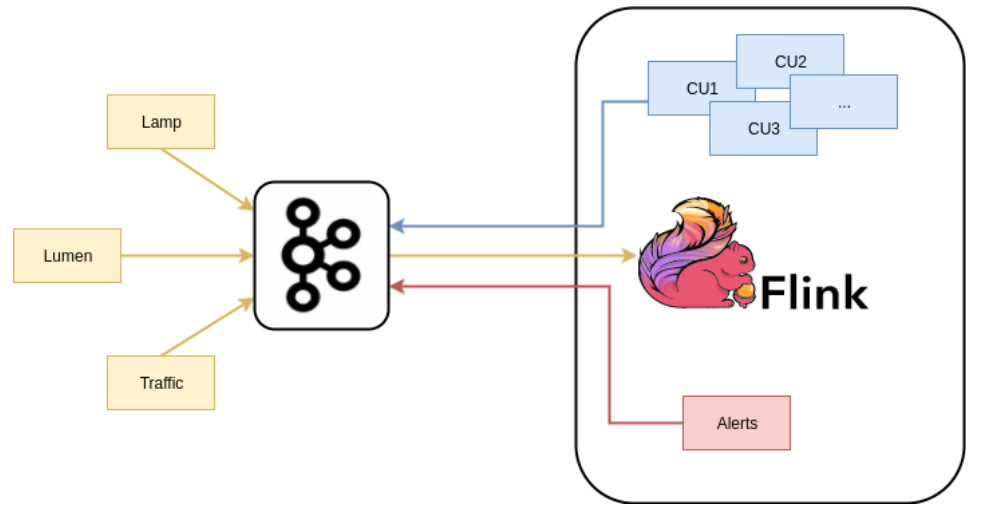
\includegraphics[scale=0.50]{img/ember_kafkatopology}
	\caption{Topics based messages routing}
	\label{fig:ember_kafkatopology}
\end{center}
\end{figure}

\section{Message oriented approach}
Apache Kafka plays its MOM role connecting all the components of our system so let’s see how they are related to each other thanks to it (\hyperref[fig:ember_kafkatopology]{figure 5}): control units and Flink produce a lot of data in streams that are organized in topics: lamps, lumens and traffic, being specific. A system such as this can be sufficient but let’s think: being a smart lamps grid the system has to emit orders directed to a single lamp among thousands. Kafka can manage runtime topics creation but a topic for each lamp is meaningless and inefficient; requiring the data stream processing system to know the right position of the lamp among network is infeasible as well. Let we analyze better the problem.

\subsection{Sensors to Kafka}
Lamps are supposed to be given, with a micro-controller built inside them capable to connect to the city intranet, to understand the power level proper of the bulb model and how such parameters relates one another in order to obtain the right luminosity. A lamp produce a JSON formatted string containing: the lamp id, the model of the light bulb, the timestamp of the last replacement instant of time, the current power consumption, the luminosity level, the control unit where it is registered, etc.

The lumen sensor is placed upon the street lamp and is managed by the same micro-controller; lumen sensors common for entire streets are managed as well. The lumen produce a JSON formatted string containing the same id of the lamp where it is placed upon (or a nonce for the common sensors), the luminosity value recorded, the street where it is located and the timestamp of the time instant when the data has been recorded.

The traffic sensor is realized by third party APIs and it is registered to Kafka producing a JSON formatted string containing the street monitored, the traffic value and the timestamp of the recorded time.

\subsection{Kafka to Adapters}
Once Flink calculates the state a street lamp should have it sends control directives to custom topics. Each lamps, in fact, is linked to a control unit and this information is included in the JSON sent by lamps to the system. That’s where the control directive is routed, a topic that is identified by the string that identify the control unit responsible of a particular street lamp; so we can, on one hand, free Kafka of an incredible number of topics and, on the other hand, free smart lamps to register themselves on their ones. As we said even the alerts of lamps not functioning or not communicating for a too long time can be routed to Kafka. Such alarms are simply transmitted to it using the connector provided by Flink that requires a byte encoding of the Alert object and the specification of the topic where they are directed to, a custom module can be easily engineered via a Kafka consumer to handle the alerts properly (our project let the user specify via configuration file to store the alerts into Elasticsearch instead).

\subsection{Control feedback}
Each lamps is registered to a particular control unit (we will cover how in the next section), which takes care to register itself to the topic of its own, so it can read the responses and understands to which lamp direct them. Once the response will be made available the control unit reads the messages and convert them to a JSON object so it can access their attributes; it determines the id of the lamp and check in the Redis database to find the IP address related to that lamp id. That’s the core of the indirection level of the whole architecture. Kafka and the control unit makes possible all of this, making our system totally plug and play for a better large scale deployment.


\section{THE CITY GRID}

\subsection{Local streetlamps control}
% TODO review
We needed a web server component capable of directing lamps data to Kafka and directive from Flink to lamps. The control unit, codenamed Metropolis, has been built with such purpose in mind giving us the possibility to create a new indirection level that is placed among lamps and Kafka/Flink. Lamps talks to the control unit which maintains a mapping between the lamps IDs and their IP addresses inside the local city network. Lamps have to be registered to the right control unit in order to submit their data inside the system which increases the security level of our system (once placed, the lamp has to be registered by the local control unit, which could manage a street or a district; such operation needs to be done by an operator that places the lamp). The control unit validates the lamps and sends their data to the Kafka lamp topic. 
\subsection{Control units at scale}
To scale this solution and to integrate this kind of grid, we provided each control unit with a RESTful API to register new lamps, retrieve statistics and to interact with them lamp themselves using a plug-and-play paradigm: once the lamp is registered it has only to contact with a record the control unit to receive then regularly a control feedback from the processing system. 

In addiction an external project, based on AWS Lambda\footnote{To learn more visit: aws.amazon.com/lambda} functions as microservices platform, to provide a unique scalable directory for control units registration and retrieval using a geo-query on Elasticsearch. It allows third party APIs to retrieve control units per-area or per-city and then to access them directly. 
 
\section{TESTS AND PERFORMANCES}
It is clear that Project Ember has a lot of different metrics upon which can be made performances analysis. Proceeding with the validation of our architecture we conducted a lot of tests to ensure the forwarding operation between operators different in API concepts and in behavior (think of the difference between the Kafka consumer as a source, the alerts query on Elasticsearch, the Kafka producers as sinks etc.). In this section we will cover what we think are the most important metrics to face when deploying this system at scale, as well as the configuration we used to produce the data you can appreciate in \hyperref[fig:ember_metrics]{figure 6}.

\begin{figure}
\begin{subfigure}{.5\textwidth}
	\centering
	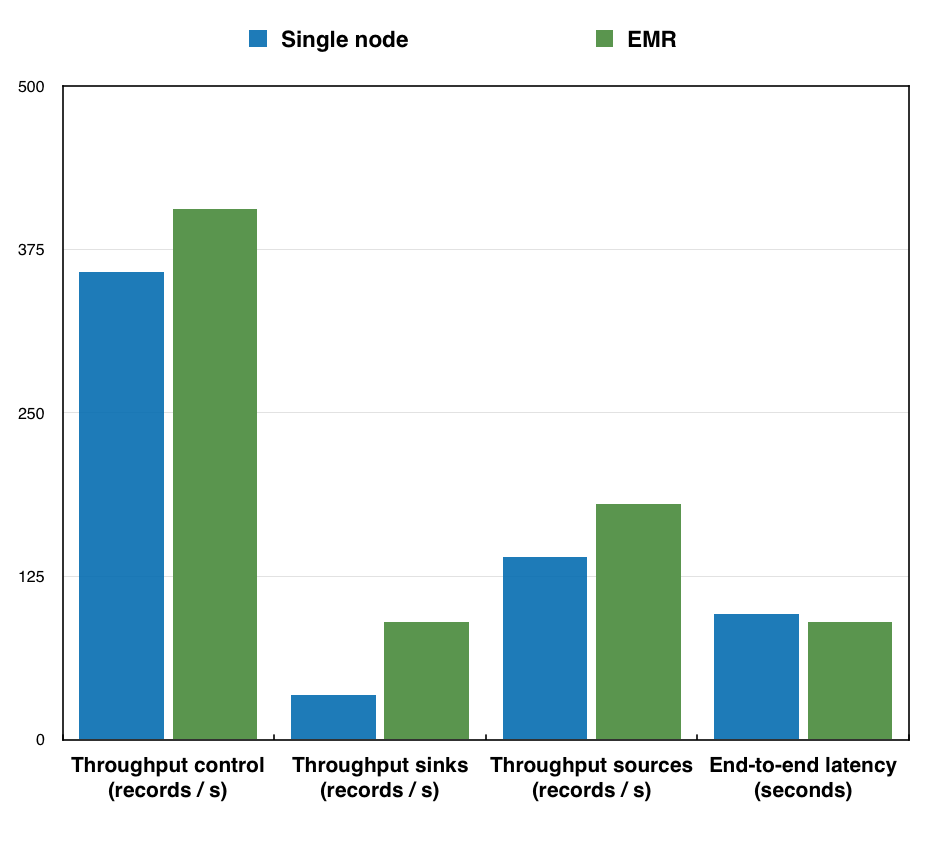
\includegraphics[scale=0.50]{img/ember_chart}
	\caption{Performances metrics comparison}
	\label{fig:ember_chart}
\end{subfigure}

\begin{subfigure}{.5\textwidth}
	\centering
	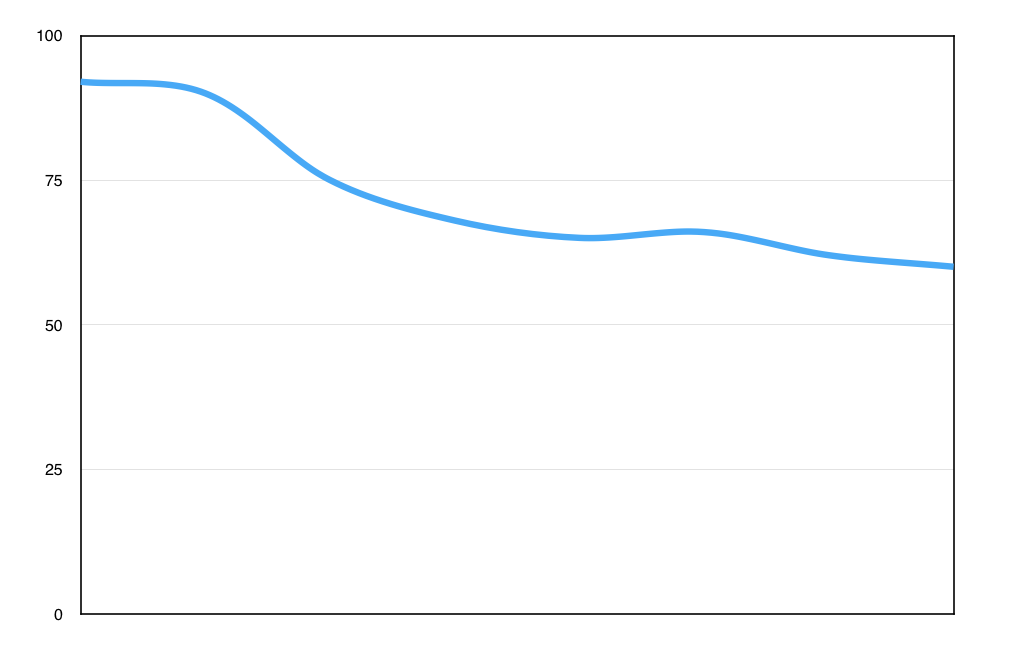
\includegraphics[scale=0.50]{img/ember_chart_latency}
	\caption{End-to-end latency (seconds) - transient analysis}
	\label{fig:ember_chart_latency}
\end{subfigure}
\caption{Project Ember operational performances}
\label{fig:ember_metrics}
\end{figure}

\subsection{The city simulator}
There are two way to test a project of this kind: testing just the stream processing topology producing a fake data source or simulating the entire grid. The latter was our choice.

We developed a "city simulator", configurable and customizable: a multithreaded Python console application capable of simulating the behavior of thousands of lamps. The values produced are typical of a grid of lamps and sensors across a day-long span, with different lumen levels according to the height of the sun (via a simple sin wave), with random traffic percentage registered for each street, different values for lamps models and a rumored measure introduced to simulate consumption levels.

The simulator, codenamed Tomorrowland, in this configuration, sends to actually deployed control units data comparable with those of a small district of a typical Italian city. In particular, in the tests we will have two thousands lamps from one hundred different locations, transmitting to their control unit every ten seconds, and two thousands lumen level records sent directly to the Kafka cluster with one hundred records describing traffic average on the different streets. 

\subsection{Testing environment}
We adopted two configurations to test the architecture performances. Both of them used a replicated cluster of Apache Kafka nodes and a small cluster for Elasticsearch. Both of them were deployed using the AWS EC2 cloud service\footnote{Amazon Web Services, Elastic Compute Cloud - aws.amazon.com/ec2} offered by the Amazon Student Grant. 
In particular [...]

\subsection{Metrics}



\section{NEXT STEPS AND CONCLUSIONS}

\subsection{Security}

\subsection{Deployment}

\subsection{Conclusions}

\section*{Repository}
The Project Ember official homepage, with guides and code to deploy and customize each component described in this paper, is available at: \href{https://github.com/projectember}{github.com/projectember}. Fork us!

